\section{Question 2}
   \subsection{Part a}
        \hspace*{0.6cm}\textbf{Reconstruct lại hình sử dụng 1 và 3 eigen value lớn nhất bằng tay và lập trình Reconstruct lại hình sử
dụng 1 và 3 eigen value lớn nhất sử dụng hàm opencv }
        \begin{align*}
            X = \begin{bmatrix}
            0 & 0 & 0 & 255 & 0 & 0 & 0 \\
            0 & 255 & 0 & 255 & 0 & 0 & 0 \\
            0 & 255 & 255 & 255 & 255 & 0 & 0 \\
            0 & 0 & 255 & 255 & 255 & 255 & 0 \\
            0 & 255 & 255 & 255 & 255 & 0 & 0 \\
            0 & 255 & 0 & 255 & 0 & 0 & 0 \\
            0 & 0 & 0 & 255 & 0 & 0 & 0
            \end{bmatrix}
        \end{align*}
        \subsubsection{Tính tay}
            \begin{itemize}
                \item \textbf{Buớc 1: Tính kỳ vọng của dữ liệu theo hàng:}
                    \begin{align}
                        \mu_x = \frac{1}{N}\sum_{i=1}^{N}x_i
                    \end{align}
                    Với N = 7, ta có:
                    \begin{align*}
                        \mu_x = \begin{bmatrix}
                            36.42857 & 72.85714 & 145.71428 & 145.71428 & 145.71428 & 72.85714 & 36.42857 
                        \end{bmatrix}
                    \end{align*}
                \item \textbf{Buớc 2: Trừ mỗi điểm của dữ liệu với vector kỳ vọng, ta đuợc ma trận A:}
                    \begin{align*}
                        A = \begin{bmatrix}
                        -36.429 & -36.429 & -36.429 & 218.571 & -36.429 & -36.429 & -36.429 \\
                        -72.857 & 182.143 & -72.857 & 182.143 & -72.857 & -72.857 & -72.857 \\
                        -145.714 & 109.286 & 109.286 & 109.286 & 109.286 & -145.714 & -145.714 \\
                        -145.714 & -145.714 & 109.286 & 109.286 & 109.286 & 109.286 & -145.714 \\
                        -145.714 & 109.286 & 109.286 & 109.286 & 109.286 & -145.714 & -145.714 \\
                        -72.857 & 182.143 & -72.857 & 182.143 & -72.857 & -72.857 & -72.857 \\
                        -36.429 & -36.429 & -36.429 & 218.571 & -36.429 & -36.429 & -36.429
                        \end{bmatrix}
                    \end{align*}
                \item \textbf{Buớc 3: Tính ma trận hiệp phương sai C:}
                    \begin{align}
                        C = \frac{1}{N-1}AA^T
                    \end{align}
                    \begin{align*}
                        C = \begin{bmatrix}
                        9289.284 & 7741.072 & 4644.643 & 4644.643 & 4644.643 & 7741.072 & 9289.284 \\
                        7741.072 & 15482.142 & 9289.284 & -1548.214 & 9289.284 & 15482.142 & 7741.072 \\
                        4644.643 & 9289.284 & 18578.570 & 7741.071 & 18578.570 & 9289.284 & 4644.643 \\
                        4644.643 & -1548.214 & 7741.071 & 18578.570 & 7741.071 & -1548.214 & 4644.643 \\
                        4644.643 & 9289.284 & 18578.570 & 7741.071 & 18578.570 & 9289.284 & 4644.643 \\
                        7741.072 & 15482.142 & 9289.284 & -1548.214 & 9289.284 & 15482.142 & 7741.072 \\
                        9289.284 & 7741.072 & 4644.643 & 4644.643 & 4644.643 & 7741.072 & 9289.284
                        \end{bmatrix}
                    \end{align*}
                \item \textbf{Buớc 4: Tính các giá trị riêng và vector riêng của ma trận hiệp phương sai C. }
                    \begin{align}
                        A \mathbf{v} = \boldsymbol{\lambda} \mathbf{v}
                    \end{align}
                    Với $\boldsymbol{\lambda}$ là giá trị riêng và $\mathbf{v}$ là vector riêng tương ứng.\\
                    \begin{lstlisting}
eigvals, eigvecs = np.linalg.eigh(covariance_matrix)
                    \end{lstlisting}
                    Dùng hàm \texttt{numpy.linalg.eig()} trong python để tìm Eigenvalues và Eigenvectors ta có:\\
                    \text{Eigenvalues:}
                    \begin{align*}
                        \boldsymbol{\lambda} = \begin{bmatrix}
                        61813.695 & 25143.047 & 15744.729 & 2577.094 & 0 & 0 & 0
                        \end{bmatrix}^T
                    \end{align*}
                    \text{Eigenvectors:}
                    \begin{align*}
                        \mathbf{V} = \begin{bmatrix}
                        -0.274 & -0.102 & -0.502 & 0.403 & 0.625 & 0.175 & -0.281 \\
                        -0.417 & -0.416 & -0.003 & -0.392 & -0.329 & 0.397 & -0.484 \\
                        -0.481 & 0.273 & 0.383 & 0.219 & -0.038 & -0.558 & -0.433 \\
                        -0.201 & 0.696 & -0.450 & -0.522 & 0 & 0 & 0 \\
                        -0.481 & 0.273 & 0.383 & 0.219 & 0.038 & 0.558 & 0.433 \\
                        -0.417 & -0.416 & -0.003 & -0.392 & 0.329 & -0.397 & 0.484 \\
                        -0.274 & -0.102 & -0.502 & 0.403 & -0.625 & -0.175 & 0.281
                        \end{bmatrix}
                    \end{align*}
                \item \textbf{Buớc 5: Chọn Eigenvectors ứng với Eigenvalues lớn nhất:}
                    \begin{itemize}
                        \item Trường hợp 1 eigenvalue lớn nhất:
                            \begin{align*}
                                \mathbf{v_1} = \begin{bmatrix}
                                -0.274 \\
                                -0.417 \\
                                -0.481 \\
                                -0.201 \\
                                -0.481 \\
                                -0.417 \\
                                -0.274
                                \end{bmatrix}
                            \end{align*}
                        \item Trường hợp 3 eigenvalues lớn nhất:
                            \begin{align*}
                                \mathbf{V}_{1:3} = 
                                \begin{bmatrix}
                                -0.274 & -0.102 & -0.502 \\
                                -0.417 & -0.416 & -0.003 \\
                                -0.481 & 0.273 & 0.383 \\
                                -0.201 & 0.696 & -0.450 \\
                                -0.481 & 0.273 & 0.383 \\
                                -0.417 & -0.416 & -0.003 \\
                                -0.274 & -0.102 & -0.502
                                \end{bmatrix}
                            \end{align*}
                    \end{itemize}
                \item \textbf{Buớc 6: Chiếu dữ liệu vào không gian PCA:}
                    \begin{align}
                        Z = U_k^T X_{\text{centered}}
                    \end{align}
                    \begin{itemize}
                        \item Trường hợp 1 eigenvalue lớn nhất:
                            \begin{align*}
                                Z &= \mathbf{v_1}^T \cdot X_{\text{centered}} \nonumber \\
                                &= \begin{bmatrix}
                                250.047 & -207.600 & -46.290 & -398.679 & -46.290 & 198.765 & 250.047
                                \end{bmatrix}
                            \end{align*}
                        \item Trường hợp 3 eigenvalues lớn nhất:
                            \begin{align*}
                                Z &= \mathbf{V}_{1:3}^T \cdot X_{\text{centered}} \nonumber \\
                                &= \begin{bmatrix}
                                250.047 & -207.600 & -46.290 & -398.679 & -46.290 & 198.765 & 250.047 \\
                                -113.006 & -185.804 & 203.735 & -60.154 & 203.735 & 64.500 & -113.006 \\
                                -9.012 & 184.881 & 71.466 & -185.925 & 71.466 & -123.864 & -9.012
                                \end{bmatrix}
                            \end{align*}
                    \end{itemize}
                \item \textbf{Buớc 7: Khôi phục lại dữ liệu:}
                    \begin{itemize}
                        \item Trường hợp 1 eigenvalue lớn nhất:
                            \begin{align*}
                                \small
                                X_{\text{reconstructed}} = \begin{bmatrix}
                                -32.112 & 93.334 & 49.117 & 145.711 & 49.117 & -18.055 & -32.112 \\
                                -31.374 & 159.395 & 92.153 & 239.045 & 92.153 & -9.998 & -31.374 \\
                                25.567 & 245.466 & 167.957 & 337.279 & 167.957 & 50.208 & 25.567 \\
                                95.429 & 187.463 & 155.023 & 225.890 & 155.023 & 105.742 & 95.429 \\
                                25.567 & 245.466 & 167.957 & 337.279 & 167.957 & 50.208 & 25.567 \\
                                -31.374 & 159.395 & 92.153 & 239.045 & 92.153 & -9.998 & -31.374 \\
                                -32.112 & 93.334 & 49.117 & 145.711 & 49.117 & -18.055 & -32.112
                                \end{bmatrix}
                            \end{align*}
                        \item Trường hợp 3 eigenvalues lớn nhất:
                            \begin{align*}
                                \small
                                X_{\text{reconstructed}} = \begin{bmatrix}
                                -16.099 & 19.440 & -7.465 & 245.137 & -7.465 & 37.550 & -16.099 \\
                                15.634 & 236.121 & 7.249 & 264.578 & 7.249 & -36.465 & 15.634 \\
                                -8.736 & 265.550 & 250.949 & 249.648 & 250.949 & 20.377 & -8.736 \\
                                20.824 & -25.146 & 264.656 & 267.757 & 264.656 & 206.429 & 20.824 \\
                                -8.736 & 265.550 & 250.949 & 249.648 & 250.949 & 20.377 & -8.736 \\
                                15.634 & 236.121 & 7.249 & 264.578 & 7.249 & -36.465 & 15.634 \\
                                -16.099 & 19.440 & -7.465 & 245.137 & -7.465 & 37.550 & -16.099
                                \end{bmatrix}
                            \end{align*}
                    \end{itemize}
                    Với threshold = 150, ta có kết quả nhị phân như sau:
                    \begin{itemize}
                        \item Trường hợp 1 eigenvalue lớn nhất:
                            \begin{align*}
                                X_{\text{binary}} = \begin{bmatrix}
                                0 & 0 & 0 & 0 & 0 & 0 & 0 \\
                                0 & 255 & 0 & 255 & 0 & 0 & 0 \\
                                0 & 255 & 255 & 255 & 255 & 0 & 0 \\
                                0 & 255 & 255 & 255 & 255 & 0 & 0 \\
                                0 & 255 & 255 & 255 & 255 & 0 & 0 \\
                                0 & 255 & 0 & 255 & 0 & 0 & 0 \\
                                0 & 0 & 0 & 0 & 0 & 0 & 0
                                \end{bmatrix}
                            \end{align*}
                        \item Trường hợp 3 eigenvalues lớn nhất:
                            \begin{align*}
                                X_{\text{binary}} = \begin{bmatrix}
                                0 & 0 & 0 & 255 & 0 & 0 & 0 \\
                                0 & 255 & 0 & 255 & 0 & 0 & 0 \\
                                0 & 255 & 255 & 255 & 255 & 0 & 0 \\
                                0 & 0 & 255 & 255 & 255 & 255 & 0 \\
                                0 & 255 & 255 & 255 & 255 & 0 & 0 \\
                                0 & 255 & 0 & 255 & 0 & 0 & 0 \\
                                0 & 0 & 0 & 255 & 0 & 0 & 0
                                \end{bmatrix}
                            \end{align*}
                    \end{itemize}
            \end{itemize}
        \subsubsection{Lập trình với OpenCV}
            \begin{itemize}
                \item \textbf{Buớc 1: Khai báo các thư viện và ma trận ảnh ban đầu:}
                \begin{lstlisting}
import numpy as np
import cv2

image = np.array([
        [0, 0, 0, 255, 0, 0, 0],
        [0, 255, 0, 255, 0, 0, 0],
        [0, 255, 255, 255, 255, 0, 0],
        [0, 0, 255, 255, 255, 255, 0],
        [0, 255, 255, 255, 255, 0, 0],
        [0, 255, 0, 255, 0, 0, 0],
        [0, 0, 0, 255, 0, 0, 0],
    ], dtype=np.float32)
                \end{lstlisting}
                \item \textbf{Buớc 2: Tính mean và eigenvectors sử dụng OpenCV \texttt{PCACompute}:}
                \begin{lstlisting}
mean, eigenvectors = cv2.PCACompute(image, mean=None, maxComponents=num_components)
                \end{lstlisting}
                \item \textbf{Buớc 3: Giảm chiều dữ liệu sử dụng OpenCV \texttt{PCAProject}:}
                \begin{lstlisting}
Z = cv2.PCAProject(image, mean, eigenvectors) 
                \end{lstlisting}
                \item \textbf{Buớc 4: Phục hồi lại ảnh sử dụng OpenCV \texttt{PCABackProject}:}
                \begin{lstlisting}
X_reconstructed = cv2.PCABackProject(Z, mean, eigenvectors) 
                \end{lstlisting}
                \begin{itemize}
                    \item Kết quả khôi phục với 1 eigenvalue:
                    \begin{align*}
                        \small
                        X_{\text{reconstructed}} = \begin{bmatrix}
                        0 & 123.857 & -10.011 & 255.000 & -10.011 & -7.286 & 0 \\
                        0 & 127.806 & 11.540 & 255.000 & 11.540 & 0.611 & 0 \\
                        0 & 170.909 & 246.797 & 255.000 & 246.797 & 86.817 & 0 \\
                        0 & 174.857 & 268.349 & 255.000 & 268.349 & 94.714 & 0 \\
                        0 & 170.909 & 246.797 & 255.000 & 246.797 & 86.817 & 0 \\
                        0 & 127.806 & 11.540 & 255.000 & 11.540 & 0.611 & 0 \\
                        0 & 123.857 & -10.011 & 255.000 & -10.011 & -7.286 & 0
                        \end{bmatrix}
                    \end{align*}
                    
                    Sau khi áp dụng threshold $\geq$ 150:
                    \begin{align*}
                        X_{\text{binary}} = \begin{bmatrix}
                        0 & 0 & 0 & 255 & 0 & 0 & 0 \\
                        0 & 0 & 0 & 255 & 0 & 0 & 0 \\
                        0 & 255 & 255 & 255 & 255 & 0 & 0 \\
                        0 & 255 & 255 & 255 & 255 & 0 & 0 \\
                        0 & 255 & 255 & 255 & 255 & 0 & 0 \\
                        0 & 0 & 0 & 255 & 0 & 0 & 0 \\
                        0 & 0 & 0 & 255 & 0 & 0 & 0
                        \end{bmatrix}
                    \end{align*}
                    
                \item Kết quả khôi phục với 3 eigenvalues:
                    \begin{align*}
                        \small
                        X_{\text{reconstructed}} = \begin{bmatrix}
                        0 & 0 & 0 & 255 & 0 & 0 & 0 \\
                        0 & 255 & 0 & 255 & 0 & 0 & 0 \\
                        0 & 255 & 255 & 255 & 255 & 0 & 0 \\
                        0 & 0 & 255 & 255 & 255 & 255 & 0 \\
                        0 & 255 & 255 & 255 & 255 & 0 & 0 \\
                        0 & 255 & 0 & 255 & 0 & 0 & 0 \\
                        0 & 0 & 0 & 255 & 0 & 0 & 0
                        \end{bmatrix}
                    \end{align*}
                    
                    \textit{Lưu ý: Các giá trị rất nhỏ ($\approx 10^{-5}$) được làm tròn về 0}
                    
                    Sau khi áp dụng threshold $\geq$ 150:
                    \begin{align*}
                        X_{\text{binary}} = \begin{bmatrix}
                        0 & 0 & 0 & 255 & 0 & 0 & 0 \\
                        0 & 255 & 0 & 255 & 0 & 0 & 0 \\
                        0 & 255 & 255 & 255 & 255 & 0 & 0 \\
                        0 & 0 & 255 & 255 & 255 & 255 & 0 \\
                        0 & 255 & 255 & 255 & 255 & 0 & 0 \\
                        0 & 255 & 0 & 255 & 0 & 0 & 0 \\
                        0 & 0 & 0 & 255 & 0 & 0 & 0
                        \end{bmatrix}
                    \end{align*}
                \end{itemize}
            \end{itemize}
        \subsubsection{Nhận xét}
            \textbf{Nhận xét về kết quả thu được khi sử dụng 1 và 3 eigen value lớn nhất để reconstruct lại hình ảnh:}
            \begin{itemize}
                \item Với việc sử dụng 1 eigenvector lớn nhất để khôi phục lại ảnh, ta chỉ có thể giữ lại được những đặc trưng cơ bản nhất của ảnh gốc. Kết quả nhị phân thu được có nhiều điểm bị mất thông tin so với ảnh gốc ban đầu.
                \item Khi sử dụng 3 eigenvectors lớn nhất, kết quả khôi phục lại ảnh gần như giống hệt với ảnh gốc ban đầu. Kết quả nhị phân thu được cũng giữ lại được hầu hết các đặc trưng quan trọng của ảnh gốc.
                \item Điều này cho thấy rằng việc chọn số lượng eigenvectors sử dụng trong PCA ảnh hưởng trực tiếp đến chất lượng của ảnh khôi phục và khả năng giữ lại thông tin quan trọng từ dữ liệu gốc.
            \end{itemize}
            \textbf{So sánh kết quả thu được giữa việc tính PCA bằng tay và sử dụng hàm OpenCV:}
            \begin{itemize}
                \item Kết quả khôi phục lại ảnh từ cả hai phương pháp (tính PCA bằng tay và sử dụng hàm OpenCV) đều cho ra các ma trận ảnh tương tự nhau, đặc biệt là khi sử dụng 3 eigenvectors lớn nhất.
                \item Sự khác biệt nhỏ xuất phát từ cách OpenCV tổ chức dữ liệu đầu vào, cụ thể OpenCV mặc định coi mỗi hàng là một sample và mỗi cột là một thuộc tính (feature). Trong khi đó, phần tính tay ta đã coi mỗi cột là một sample và mỗi hàng là một thuộc tính.
            \end{itemize}
    \newpage
    \subsection{Part b}
            \hspace*{0.6cm}\textbf{Cho hình sau hãy nén hình sử dụng số lượng eigen ít nhất có thể:}
            \begin{figure}[H]
                \centering
                
\includegraphics[width=0.5\textwidth]{pictures/section2/s2_p1_Original_Image}
                \caption{Hình ảnh gốc}
                \label{fig:original_image}
            \end{figure}
        \subsubsection{Ý tưởng}
            \hspace*{0.6cm}Ta sẽ sử dụng OpenCV để thực hiện PCA trên hình ảnh đã cho. Do không biết số lượng eigenvectors cần sử dụng để nén hình ảnh, ta sẽ áp dụng phương pháp chọn số lượng eigenvectors dựa trên ngưỡng tỷ lệ phương sai từ đồ thị \textit{cumulative explained variance} và thêm một tiêu chí \textit{elbow heuristic} để tự động xác định số thành phần chính $k$ tối ưu.
        \subsubsection{Các buớc thực hiện}
            \begin{itemize}
                \item \textbf{Bước 1: Đọc ảnh và chuẩn bị dữ liệu}

                    Ảnh xám đầu vào được đọc bằng OpenCV và biểu diễn dưới dạng ma trận $X \in \mathbb{R}^{H \times W}$. 
                    Mỗi hàng của ảnh được coi là một sample, mỗi cột là một thuộc tính (feature).
                    Dữ liệu được chuyển sang kiểu \texttt{float32} để phù hợp với hàm PCA của OpenCV.
                    \begin{lstlisting}
image_path = 'Question_2/image.png'
img = cv2.imread(image_path, cv2.IMREAD_GRAYSCALE)
                    \end{lstlisting}
                \item \textbf{Bước 2: Thực hiện PCA bằng OpenCV}

                    Sử dụng hàm \texttt{cv2.PCACompute} để tính vector trung bình $\boldsymbol{\mu}$ và các eigenvectors:
                    \begin{align}
                        \boldsymbol{\mu}, \mathbf{V} = \texttt{PCACompute}(X)
                    \end{align}
                    Sau đó, dữ liệu được chiếu sang không gian PCA bằng hàm \texttt{cv2.PCAProject}:
                    \begin{align}
                        Z = (X - \boldsymbol{\mu}) \mathbf{V}^T
                    \end{align}
                    \begin{lstlisting}
mean, eigvecs = cv2.PCACompute(X, mean=None, maxComponents=max_components)
Z = cv2.PCAProject(X, mean, eigvecs)
                    \end{lstlisting}

                \item \textbf{Bước 3: Tính explained variance và cumulative explained variance}

                    Phương sai trên từng thành phần chính được tính từ ma trận $Z$:
                    \begin{align}
                        \sigma_k^2 = \mathrm{Var}(Z_k)
                    \end{align}
                    Tổng phương sai của dữ liệu gốc:
                    \begin{align}
                        \sigma_{\text{total}}^2 = \sum_{j=1}^{W} \mathrm{Var}(X_j)
                    \end{align}
                    Tỉ lệ phương sai được giải thích bởi từng thành phần chính:
                    \begin{align}
                        r_k = \frac{\sigma_k^2}{\sigma_{\text{total}}^2}
                    \end{align}
                    Phương sai tích luỹ:
                    \begin{align}
                        R_k = \sum_{i=1}^{k} r_i
                    \end{align}
                    \begin{lstlisting}
variances = np.var(Z, axis=0, ddof=1)
total_var = np.sum(np.var(X, axis=0, ddof=1))

if total_var <= 0:
    explained = np.zeros_like(variances)
else:
    explained = variances / total_var
cumulative = np.cumsum(explained)
                    \end{lstlisting}
                \item \textbf{Bước 4: Vẽ đồ thị cumulative explained variance}

                    Đồ thị $R_k$ theo số lượng thành phần chính $k$ được vẽ và lưu lại nhằm quan sát tốc độ hội tụ của phương sai.
                    Trên đồ thị có đánh dấu các ngưỡng phương sai phổ biến như $90\%$ và $95\%$.
                    \begin{lstlisting}
def plot_and_save_cumulative(cumulative, out_path, title='Cumulative explained variance'):
    plt.figure(figsize=(7,4))
    k = len(cumulative)
    x = np.arange(1, k+1)
    plt.plot(x, cumulative, marker='o', label='Cumulative explained variance')
    plt.bar(x, np.diff(np.concatenate([[0.0], cumulative])), alpha=0.3, label='Per-component')
    plt.xlabel('Number of components (k)')
    plt.ylabel('Cumulative explained variance')
    plt.ylim(0,1.05)
    plt.grid(True)
    plt.axhline(0.90, color='red', linestyle='--', linewidth=0.7)
    plt.axhline(0.95, color='green', linestyle=':', linewidth=0.7)
    plt.title(title)
    plt.legend()
    plt.tight_layout()
    plt.savefig(out_path, dpi=200)
    plt.close()
                    \end{lstlisting}
                \item \textbf{Bước 5: Chọn số lượng eigenvectors theo ngưỡng phương sai}

                    Tìm số lượng thành phần chính nhỏ nhất $k_{\text{threshold}}$ thoả mãn:
                    \begin{align}
                        R_{k_{\text{threshold}}} \ge \text{threshold}
                    \end{align}
                    với \texttt{threshold} được lựa chọn trước (ví dụ $0.9$ hoặc $0.95$).
                    \begin{lstlisting}
def choose_k_by_threshold(cumulative, threshold=0.95):
    k = int(np.searchsorted(cumulative, threshold) + 1)
    if k < 1:
        k = 1
    if k > len(cumulative):
        k = len(cumulative)
    return k
                    \end{lstlisting}
                \item \textbf{Bước 6: Chọn số lượng eigenvectors theo elbow heuristic}

                Xét đường thẳng nối giữa hai điểm $(1, R_1)$ và $(N, R_N)$ trên đồ thị phương sai tích luỹ.
                Tính khoảng cách vuông góc từ mỗi điểm $(k, R_k)$ đến đường thẳng này.
                Giá trị $k$ ứng với khoảng cách lớn nhất được chọn làm:
                \begin{align}
                    k_{\text{elbow}} = \arg\max_k \; d(k)
                \end{align}

                \item \textbf{Bước 7: Khôi phục ảnh với số lượng eigenvectors đã chọn}

                Với mỗi giá trị $k \in \{k_{\text{threshold}}, k_{\text{elbow}}\}$:
                \begin{itemize}
                    \item Thực hiện PCA lại với \texttt{maxComponents = k}.
                    \item Chiếu dữ liệu sang không gian PCA:
                    \begin{align}
                        Z_k = (X - \boldsymbol{\mu}_k)\mathbf{V}_k^T
                    \end{align}
                    \item Khôi phục lại ảnh bằng:
                    \begin{align}
                        X_{\text{reconstructed}} = Z_k \mathbf{V}_k + \boldsymbol{\mu}_k
                    \end{align}
                \end{itemize}
                \begin{lstlisting}
def choose_k_elbow(cumulative):
    cum = np.asarray(cumulative, dtype=float)
    n = len(cum)
    if n == 0:
        return 1
    if n == 1:
        return 1
    x = np.arange(1, n+1)
    x1, y1 = 1, cum[0]
    x2, y2 = n, cum[-1]
    denom = np.hypot(x2 - x1, y2 - y1)
    if denom == 0:
        return 1
    distances = np.abs((y2 - y1) * x - (x2 - x1) * cum + x2*y1 - y2*x1) / denom
    elbow_idx = int(np.argmax(distances))
    return elbow_idx + 1
                \end{lstlisting}

                \item \textbf{Bước 8: Khôi phục ảnh với k eigenvectors }

                Tiến hành áp dụng hàm khôi phục ảnh với số lượng eigenvectors $k$ đã chọn:
                \begin{lstlisting}
def reconstruct_with_k(k):
    mean_k, eigvecs_k = cv2.PCACompute(data, mean=None, maxComponents=k)
    Z_k = cv2.PCAProject(data, mean_k, eigvecs_k)
    X_recon = cv2.PCABackProject(Z_k, mean_k, eigvecs_k)  
    X_recon_clipped = np.clip(X_recon, 0, 255).astype(np.uint8)
    return X_recon_clipped
                \end{lstlisting}
            \end{itemize}
        \newpage
        \subsubsection{Kết quả thu được}
            \begin{figure}[H]
                \centering
                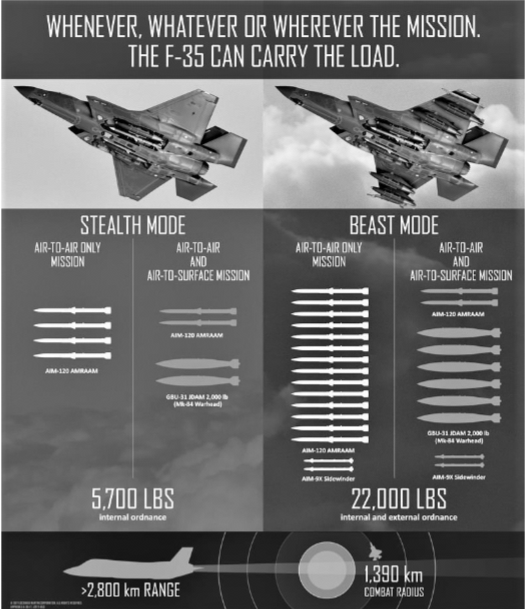
\includegraphics[width=0.6\textwidth]{pictures/section2/s2_p2_Original_Image_Grayscale.png}
                \caption{Hình ảnh gốc dưới dạng ảnh xám}
                \label{fig:original_image}
            \end{figure}
            \begin{itemize}
                \item Đồ thị cumulative explained variance:
                    \begin{figure}[H]
                        \centering
                        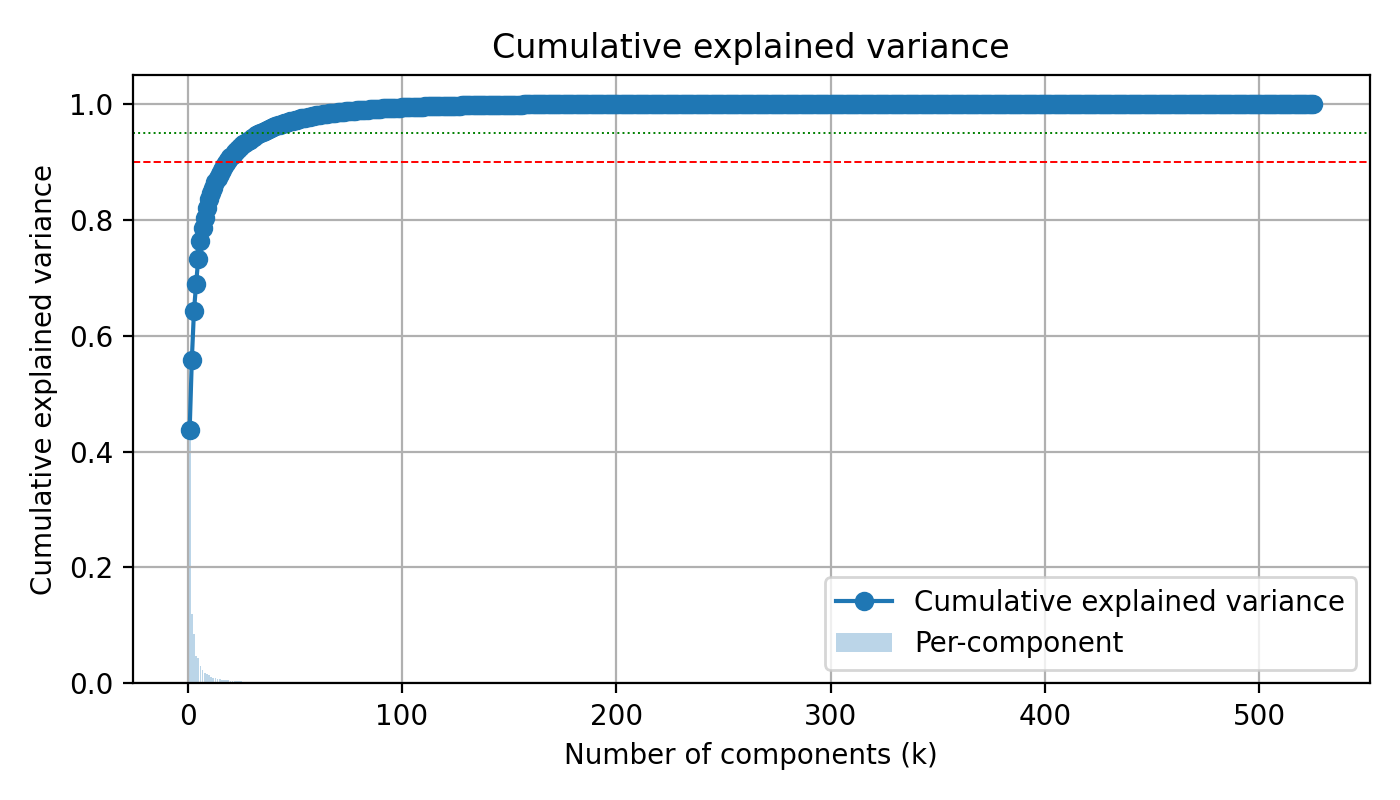
\includegraphics[width=1\textwidth]{pictures/section2/s2_p3_Cumulative_Explained_Variance.png}
                        \caption{Đồ thị cumulative explained variance}
                        \label{fig:cumulative_explained_variance}   
                    \end{figure}
                \item Kết quả khôi phục ảnh với số lượng eigenvectors theo ngưỡng phương sai 95\% ($k=35$):
                    \begin{figure}[H]
                        \centering
                        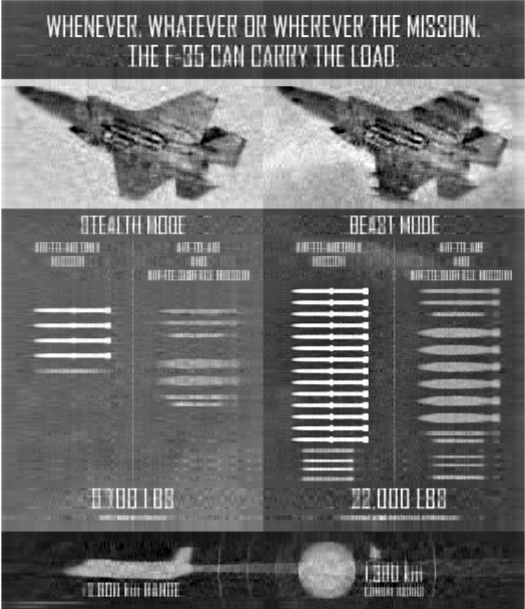
\includegraphics[width=0.5\textwidth]{pictures/section2/s2_p4_Reconstructed_Image_Threshold_95.png}
                        \caption{Ảnh khôi phục với $k=35$ (ngưỡng 95\%)}
                        \label{fig:reconstructed_image_threshold_95}
                    \end{figure}
                \item Kết quả khôi phục ảnh với số lượng eigenvectors theo ngưỡng phương sai 100\% ($k=299$):
                    \begin{figure}[H]
                        \centering
                        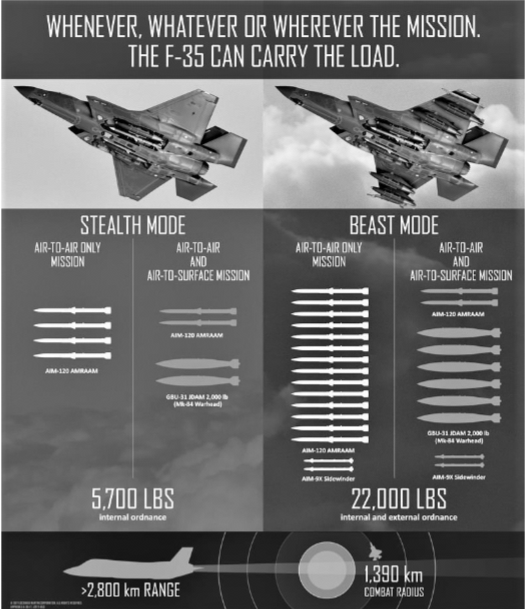
\includegraphics[width=0.5\textwidth]{pictures/section2/s2_p5_Reconstructed_Image_Threshold_100.png}
                        \caption{Ảnh khôi phục với $k=299$ (ngưỡng 100\%)}
                        \label{fig:reconstructed_image_threshold_100}
                    \end{figure} 
                \item Kết quả khôi phục ảnh với số lượng eigenvectors theo elbow heuristic ($k=47$):
                    \begin{figure}[H]
                        \centering
                        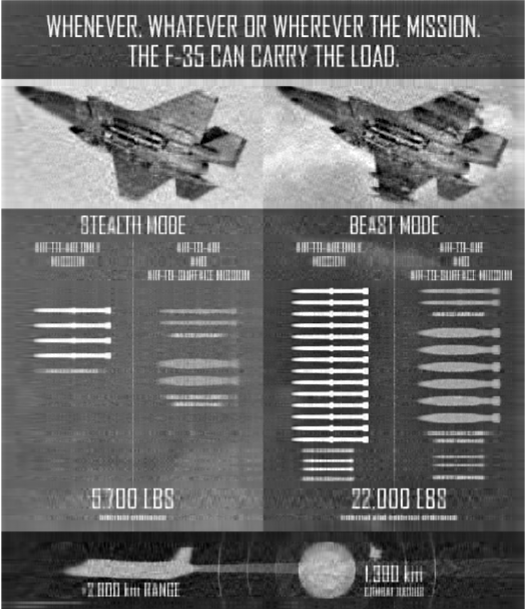
\includegraphics[width=0.5\textwidth]{pictures/section2/s2_p6_Reconstructed_Image_Elbow_Heuristic.png}
                        \caption{Ảnh khôi phục với $k=47$ (elbow heuristic)}
                        \label{fig:reconstructed_image_elbow_heuristic}
                    \end{figure}
            \end{itemize}
        \subsubsection{Nhận xét}
            \begin{itemize}
                \item Việc sử dụng ngưỡng phương sai 95\% với $k=35$ đã giúp nén ảnh đáng kể trong khi vẫn giữ được hầu hết các đặc trưng quan trọng của ảnh gốc. Kết quả khôi phục khá tốt và gần giống với ảnh gốc.
                \item Khi sử dụng ngưỡng phương sai 100\% với $k=299$, ảnh khôi phục gần như hoàn hảo so với ảnh gốc, tuy nhiên việc này không thực sự nén ảnh hiệu quả vì gần như giữ nguyên tất cả các thành phần chính.
                \item Sử dụng elbow heuristic với $k=47$ cũng mang lại kết quả khá tốt, với chất lượng ảnh khôi phục tương đương với ngưỡng 95\%. Phương pháp này tự động xác định số lượng thành phần chính tối ưu dựa trên hình dạng của đồ thị cumulative explained variance.
                \item Tổng kết lại, việc lựa chọn số lượng eigenvectors ảnh hưởng trực tiếp đến chất lượng ảnh khôi phục và khả năng nén dữ liệu. Cần cân nhắc giữa chất lượng ảnh và mức độ nén khi lựa chọn số lượng thành phần chính.    
            \end{itemize}
            
            
            